%%%%%%%%%%%%%%%%%%%%%%%%%%%%%%%%%%%%%%%%%%%%%%%%%%%%%%%%%%%%%%%%%%%%
% PREAMBLE
%%%%%%%%%%%%%%%%%%%%%%%%%%%%%%%%%%%%%%%%%%%%%%%%%%%%%%%%%%%%%%%%%%%%

\documentclass[handout]{beamer}
%\documentclass{beamer}

%------------------------------------------------------------------
% Presentation Settings
%------------------------------------------------------------------

\mode<presentation>
{
	\usetheme{Boadilla}      % or Boadilla, Singapore, ...
	\usecolortheme{default} % or albatross, beaver, crane, ...
	\usefonttheme{default}  % or serif, structurebold, ...
	\setbeamertemplate{navigation symbols}{}
	\setbeamertemplate{caption}[numbered]
	\setbeamertemplate{itemize items}[circle]
	\setbeamertemplate{itemize subitem}[triangle]
	\setbeamertemplate{enumerate items}[default]
	\setbeamerfont{caption}{size=\tiny}
	%\setbeamercolor{alerted text}{fg=blue}
}

%------------------------------------------------------------------
% Packages
%------------------------------------------------------------------
\usepackage{amsmath}
\usepackage[natbibapa]{apacite}
\usepackage{appendixnumberbeamer}
\usepackage[english]{babel}
\usepackage{comment}
\usepackage{hyperref}
\usepackage[utf8x]{inputenc}
\usepackage{pdfpages}
\usepackage{subcaption}
\usepackage{verbatim}

\usepackage{listings} % Code blocks
\usepackage{color}

\definecolor{ltgreen}{RGB}{230, 242, 230}

\lstset{frame=tb,
  language=bash,
  aboveskip=3mm,
  belowskip=3mm,
  showstringspaces=false,
  columns=flexible,
  basicstyle={\small\ttfamily},
  numbers=none,
  breaklines=true,
  breakatwhitespace=true,
  tabsize=3,
  backgroundcolor=\color{ltgreen}
}


%------------------------------------------------------------------
% Set up
%------------------------------------------------------------------

% Add section titles

\AtBeginSection[]{
	\begin{frame}
  	\vfill
  	\centering
  	\begin{beamercolorbox}[sep=8pt,center,shadow=false,rounded=false]{title}
    	\usebeamerfont{title}\insertsectionhead\par%
  	\end{beamercolorbox}
  	\vfill
  \end{frame}
}

% Reduce references font size

\renewcommand*{\bibfont}{\scriptsize}

%------------------------------------------------------------------
% Title page settings
%------------------------------------------------------------------

\title[Git/GitHub Workshop: Part 2]{Workshop: Introduction to Git and GitHub}

\subtitle{Part 2: Git Basics}

\author[P. Joly]{Philippe Joly}
\institute[FU-Berlin]{Freie Universität Berlin}

\date{March 9, 2021}

%%%%%%%%%%%%%%%%%%%%%%%%%%%%%%%%%%%%%%%%%%%%%%%%%%%%%%%%%%%%%%%%%%%%
% DOCUMENT
%%%%%%%%%%%%%%%%%%%%%%%%%%%%%%%%%%%%%%%%%%%%%%%%%%%%%%%%%%%%%%%%%%%%

\begin{document}

%------------------------------------------------------------------
% Title Page
%------------------------------------------------------------------
\begin{frame}
\titlepage
\end{frame}
%

%\begin{columns}
%  \begin{column}{0.5\textwidth}
%
%    ...
%
%  \end{column}
%  \begin{column}{0.5\textwidth}
%    ...
%  \end{column}
%\end{columns}

%%------------------------------------------------------------------

\begin{frame}{Reference}
	\begin{columns}
	
		\begin{column}{0.5\textwidth}
			\begin{itemize}
				\item This workshop draws extensively on Scott Chacon and Ben Straub (2021), \href{https://git-scm.com/book/en/v2}{\textit{ProGit}}, Version 2.1.295, 2021-02-26. 
				\item Like the book, this workshop carries the CC BY-NC-SA 3.0 license.
			\end{itemize}
		\end{column}
		
		\begin{column}{0.5\textwidth}
			\begin{figure}
				
\includegraphics[width=0.5\textwidth]{figures/progit_cover.png}
				\caption{}
			\end{figure}
		\end{column}
	
	\end{columns}
\end{frame}

%%------------------------------------------------------------------

\begin{frame}{Two ways of getting a Git repository}
	\begin{enumerate}
		\item Take a local directory that is currently not under version control and turn it into a Git repository
		\item \texttt{clone} an existing Git repository from elsewhere.
	\end{enumerate}
\end{frame}

\begin{frame}{Initializing a git repository (1)}
	\begin{itemize}
		\item Open a project folder
		\item Open your terminal from inside the project folder
		\begin{itemize}
			\item Linux (Ubuntu): right-click + open terminal here
			\item Windows: right-click + Git Bash here
			\item MacOS: you need to activate this functionality
    \end{itemize}
    \item You can otherwise navigate with the \texttt{cd} command.
  \end{itemize}
\end{frame}

\begin{frame}{Initializing a git repository (2)}
You can otherwise navigate with the \texttt{cd} command.
	\begin{exampleblock}{For Linux}
		\begin{semiverbatim}
			\item \$ cd /home/user/my\_project
		\end{semiverbatim}
  \end{exampleblock}
  \begin{exampleblock}{For MacOS}
  	\begin{semiverbatim}
  		\item \$ cd /Users/user/my\_project
  	\end{semiverbatim}
  \end{exampleblock}
  \begin{exampleblock}{For Windows}
  	\begin{semiverbatim}
  		\item \$ cd C:/Users/user/my\_project
  	\end{semiverbatim}
  \end{exampleblock}
\end{frame}

\begin{frame}{Initializing a git repository (3)}
	Now type:
	\begin{exampleblock}{}
		\begin{semiverbatim}
			\item \$ git init
		\end{semiverbatim}
	\end{exampleblock}
	\begin{itemize}
		\item Creates a subdirectory named \texttt{.git}
		\item Might be hidden depending on your configuration
		\item Your project folder is now a git repository!
	\end{itemize}
\end{frame}

\begin{frame}{Staging and committing a file}
	\begin{exampleblock}{Staging a file (taking a snapshot)}
		\begin{semiverbatim}
			\item \$ git add myfile.txt
		\end{semiverbatim}
	\end{exampleblock}
	\begin{exampleblock}{Committing a file (saving that snapshot)}
		\begin{semiverbatim}
			\item \$ git commit myfile.txt -m "Record this change in project"
		\end{semiverbatim}
	\end{exampleblock}
\end{frame}

\begin{frame}{Cloning an existing repository}
	\begin{itemize}
		\item Creates a copy of a repository stored on a remote server. 
		\item Imports the entire version history
	\end{itemize}
	\begin{exampleblock}{https protocol}
		\begin{semiverbatim}
			\item \$ git clone https://github.com/jolyphil/git-workshop
		\end{semiverbatim}
	\end{exampleblock}
	\begin{itemize}
		\item If you have set up an SSH connection on the server (here: GitHub), you can also clone the repo like this: 
	\end{itemize}
	\begin{exampleblock}{SSH protocol}
		\begin{semiverbatim}
			\item \$ git clone git@github.com:jolyphil/git-workshop
		\end{semiverbatim}
	\end{exampleblock}
	\begin{itemize}
		\item Advantage: you don't have to re-enter your username and password. 
	\end{itemize}
\end{frame}

\begin{frame}{Tip: \texttt{git clone} is usually easier than \texttt{git init}}
	\begin{itemize}
		\item \texttt{git clone} automatically sets up the connection between your local and remote repository. 
		\item You can create a repository containing only a README file on GitHub
		\begin{enumerate}
			\item Create a new repository containing only a README file on GitHub
			\item Clone this repository on your local machine
			\item Create or copy your project files into the cloned repository
			\item Start committing
		\end{enumerate}
%		\item You can proceed like this:
%		\begin{enumerate}
%			\item Log into GitHub
%			\item Click on the + sign
%			\item Click on New repository
%			\item Give a name to your repository
%			\item Click on 'Add a README file' 
%			\item Click on create repository
%			\item In your GitHub repo, click on 'Code'
%			\item Copy the SSH address
%			\item \texttt{git clone} your repository using the SSH protocol
%			\item Create or copy your local project files in the new folder
%			\item Start committing
%		\end{enumerate}
	\end{itemize}
\end{frame}

\begin{frame}{Checking the status of your files (1)}
	\begin{exampleblock}{}
		\begin{semiverbatim}
			\item \$ git status
		\end{semiverbatim}
	\end{exampleblock}
	\begin{exampleblock}{}
		\begin{semiverbatim}
			\item On branch master
			\item Your branch is up-to-date with 'origin/master'.
			\item nothing to commit, working tree clean
		\end{semiverbatim}
	\end{exampleblock}
\end{frame}

\begin{frame}{Checking the status of your files (2)}
	\begin{exampleblock}{What happens when you create or copy a file in your repo}
		\begin{semiverbatim}
			\item On branch main
			\item Your branch is up-to-date with 'origin/main'.
			\item Untracked files:
			\item (use "git add <file>..." to include in what will be committed)
			\item README
			\item nothing added to commit but untracked files present (use "git add" to track)
		\end{semiverbatim}
	\end{exampleblock}
\end{frame}

\begin{frame}{Untracked files}
	\begin{figure}
		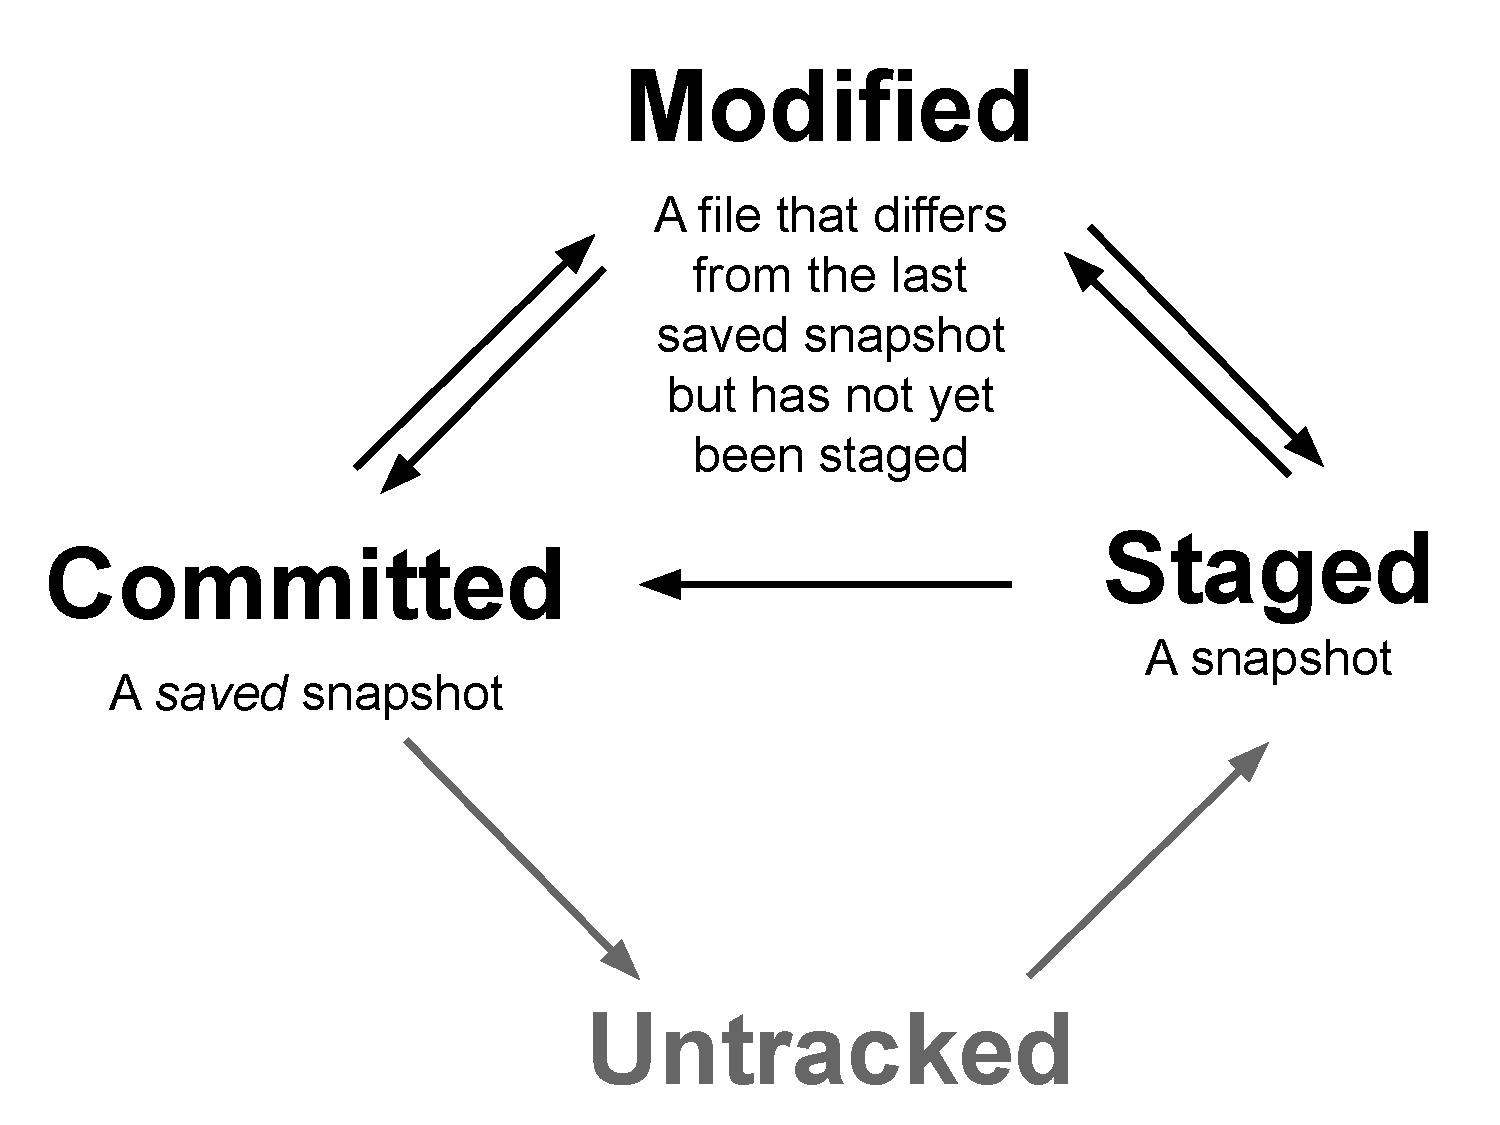
\includegraphics[width=0.8\textwidth]{figures/git_4states.pdf}
		\caption{New files have to be explicitly added to the version history.}
	\end{figure}
\end{frame}

\begin{frame}[fragile]{Tracking a new file}
Add a new file
\begin{lstlisting}
$ git add README    
\end{lstlisting}
Check the status 
\begin{lstlisting}
$ git status

On branch master
Your branch is up-to-date with 'origin/master'.
Changes to be committed:
  (use "git restore --staged <file>..." to unstage)

    new file:   README
\end{lstlisting}
\end{frame}

\begin{frame}[fragile]{Staging modified files (1)}
What happens when you modify a tracked file (here: \texttt{CONTRIBUTING.md})
\begin{lstlisting}
$ git status
On branch master
Your branch is up-to-date with 'origin/master'.
Changes to be committed:
  (use "git reset HEAD <file>..." to unstage)

    new file:   README

Changes not staged for commit:
  (use "git add <file>..." to update what will be committed)
  (use "git checkout -- <file>..." to discard changes in working directory)

    modified:   CONTRIBUTING.md
\end{lstlisting}
\end{frame}

\begin{frame}[fragile]{Staging modified files (2)}
After adding the modified file to the staging area
\begin{lstlisting}
$ git add CONTRIBUTING.md
$ git status
On branch master
Your branch is up-to-date with 'origin/master'.
Changes to be committed:
  (use "git reset HEAD <file>..." to unstage)

    new file:   README
    modified:   CONTRIBUTING.md
\end{lstlisting}
\end{frame}

\begin{frame}[fragile]{Staging modified files (3)}
What happens if you modify the file again before committing
\begin{lstlisting}
$ git status
On branch master
Your branch is up-to-date with 'origin/master'.
Changes to be committed:
  (use "git reset HEAD <file>..." to unstage)

    new file:   README
    modified:   CONTRIBUTING.md

Changes not staged for commit:
  (use "git add <file>..." to update what will be committed)
  (use "git checkout -- <file>..." to discard changes in working directory)

    modified:   CONTRIBUTING.md
\end{lstlisting}
\end{frame}

\begin{frame}[fragile]{Staging modified files (4)}
Adding the file again to the staging area.
\begin{lstlisting}
$ git add CONTRIBUTING.md
$ git status
On branch master
Your branch is up-to-date with 'origin/master'.
Changes to be committed:
  (use "git reset HEAD <file>..." to unstage)

    new file:   README
    modified:   CONTRIBUTING.md
\end{lstlisting}
\end{frame}

\begin{frame}[fragile]{Ignoring files}
You can ignore certain files by creating a \texttt{.gitignore} file in your repo. 
\begin{lstlisting}
# ignore all .a files
*.a

# but do track lib.a, even though you're ignoring .a files above
!lib.a

# only ignore the TODO file in the current directory, not subdir/TODO
/TODO

# ignore all files in any directory named build
build/

# ignore doc/notes.txt, but not doc/server/arch.txt
doc/*.txt
\end{lstlisting}
\end{frame}

\begin{frame}[fragile]{Viewing Your Staged and Unstaged Changes (1)}
Let's say you have a modified file named \texttt{CONTRIBUTING.md}
\begin{lstlisting}
$ git status
On branch master
Your branch is up-to-date with 'origin/master'.
Changes to be committed:
  (use "git reset HEAD <file>..." to unstage)

    modified:   README

Changes not staged for commit:
  (use "git add <file>..." to update what will be committed)
  (use "git checkout -- <file>..." to discard changes in working directory)

    modified:   CONTRIBUTING.md
\end{lstlisting}
\end{frame}

\begin{frame}[fragile]{Viewing Your Staged and Unstaged Changes (2)}
Compares your working directory with the staged area (or with the last commit if you haven't staged anything since then.)
\begin{lstlisting}
$ git diff
\end{lstlisting}
If you want to compare what is currently staged with the last commit, you can proceed as follows:
\begin{lstlisting}
$ git diff --staged
\end{lstlisting}
This describes what will go into your next commit. 
\end{frame}

\begin{frame}[fragile]{Committing}
This will open your default editor and let you write a commit message.
\begin{lstlisting}
$ git commit
\end{lstlisting}
It's easier to you use the \texttt{-m} option and do everything in a single command.
\begin{lstlisting}
$ git commit -m "Story 182: fix benchmarks for speed"
[master 463dc4f] Story 182: fix benchmarks for speed
 2 files changed, 2 insertions(+)
 create mode 100644 README
\end{lstlisting}
Good commit messages are important
\begin{itemize}
	\item Short, approx. 50 characters
	\item Use the imperative (e.g., "Fix this problem")
\end{itemize}
\end{frame}

\begin{frame}{What happens when you commit (1)}
	\begin{figure}
		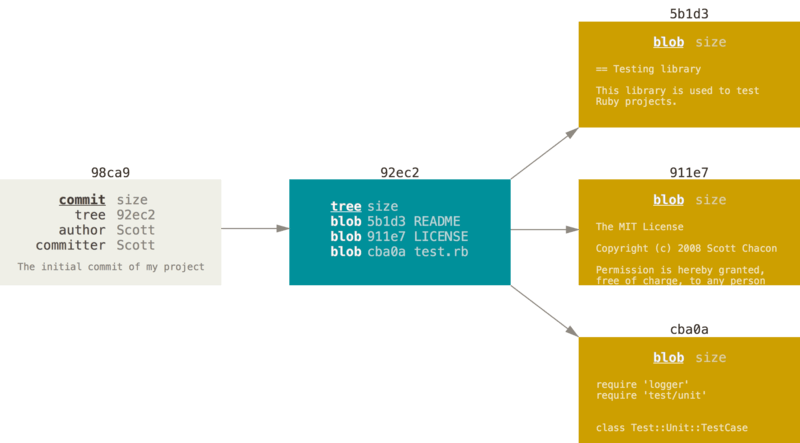
\includegraphics[width=0.9\textwidth]{figures/fig09_commit.png}
		\caption{A commit and its tree. \textit{Source}: Chacon \& Straub (2021), fig. 9.}
	\end{figure}
\end{frame}

\begin{frame}{What happens when you commit (2)}
	\begin{figure}
		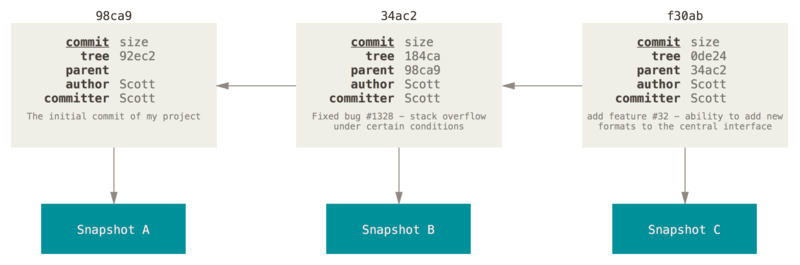
\includegraphics[width=0.9\textwidth]{figures/fig10_commits_parents.png}
		\caption{Commits and their parents. \textit{Source}: Chacon \& Straub (2021), fig. 10.}
	\end{figure}
\end{frame}

\begin{frame}[fragile]{Removing and moving files}
Removing a file
\begin{lstlisting}
$ git rm PROJECTS.md
\end{lstlisting}
Moving (renaming) a file
\begin{lstlisting}
$ git mv file_from file_to
\end{lstlisting}
Note: these operations can also be done manually in your file browser and then staged using \texttt{git add}.
\end{frame}

\begin{frame}{Exercise 1}
	\begin{enumerate}
		\item Create a new folder.
		\item Turn this folder into a Git repository using \texttt{git init}.
		\item Create a file named \texttt{README.md} inside your repo.
		\item Check the status of your git repository using \texttt{git status}.
		\item Start tracking \texttt{README.md} using \texttt{git add}.
		\item Check the status of your git repository again.
		\item Modify \texttt{README.md} using a text editor (add a line of text for example).
		\item Save \texttt{README.md}.
		\item Check the status of your git repository again.
		\item Examine the changes you have introduced using \texttt{git diff}.
		\item Stage \texttt{README.md} using \texttt{git add} again. 
		\item Commit your changes using \texttt{git commit -m}
	\end{enumerate}
\end{frame}

\begin{frame}[fragile]{Viewing the commit history}
\begin{lstlisting}
$ git log
commit ca82a6dff817ec66f44342007202690a93763949
Author: Scott Chacon <schacon@gee-mail.com>
Date:   Mon Mar 17 21:52:11 2008 -0700

    Change version number

commit 085bb3bcb608e1e8451d4b2432f8ecbe6306e7e7
Author: Scott Chacon <schacon@gee-mail.com>
Date:   Sat Mar 15 16:40:33 2008 -0700

    Remove unnecessary test
    
commit a11bef06a3f659402fe7563abf99ad00de2209e6
Author: Scott Chacon <schacon@gee-mail.com>
Date:   Sat Mar 15 10:31:28 2008 -0700

    Initial commit
\end{lstlisting}
\end{frame}

\begin{frame}[fragile]{Unstaging a staged file}
Let's say you would like to unstage \texttt{README.md}
\begin{lstlisting}
$ git status
On branch main
Changes to be committed:
  (use "git restore --staged <file>..." to unstage)
	modified:   README.md
\end{lstlisting}
\texttt{git status} already tells you what you should do.
\begin{lstlisting}
git restore --staged README.md
\end{lstlisting}
\end{frame}

\begin{frame}[fragile]{Unmodifying a modified file}
Now \texttt{README.md} is unstaged but still modified in your working directory. 
\begin{lstlisting}
$git status
On branch main
Changes not staged for commit:
  (use "git add <file>..." to update what will be committed)
  (use "git restore <file>..." to discard changes in working directory)
	modified:   README.md
\end{lstlisting}
To revert to the last committed version of this file, follow the instructions in \texttt{git status}:
\begin{lstlisting}
git restore README.md
\end{lstlisting}
\alert{Danger zone}: \texttt{git restore} will wipe out all the uncommitted changes.
\end{frame}

\begin{frame}{Exercise 2}
	\begin{enumerate}
		\item Go into the repository you created in Exercise 1
		\item Examine your commit history using \texttt{git log}.
		\item Modify \texttt{README.md} (add a line of text).
		\item Stage \texttt{README.md} using \texttt{git add}. 
		\item Check the status of your repo using \texttt{git status}. 
		\item Unstage \texttt{README.md} using \texttt{git restore --staged}.
		\item Check the status of your repo using \texttt{git status} again. 
		\item Unmodify \texttt{README.md} using \texttt{git restore}.
	\end{enumerate}
\end{frame}

\end{document}



